\documentclass[a4paper,twoside,12pt,DIV=13,BCOR=5mm,numbers=noenddot,cleardoublepage=empty]{scrbook}

\input{format}  			% File mit den benötigten Packeten, den Formatanweisungen und den Befehlsdefinitionen

\usepackage{nicefrac}
\usepackage{pgfplots}
\pgfplotsset{compat=1.18} % Set compatibility

\usepgfplotslibrary{external}
% \tikzexternalize[prefix=pictures/tikz/, shell escape=-enable-write18,optimize command away=\includepdf]

\usepackage{pgfplotstable}

\usepackage[
  output-decimal-marker={.},
  exponent-product=\cdot,
]{siunitx}
% \DeclareSIUnit \vpp {\ensuremath{\mathrm{V_{pp}}}}

\usepackage{booktabs}
\usepackage{threeparttable}
\usepackage{multirow}
\usepackage{subcaption}


\begin{document}

\renewcommand{\baselinestretch}{1.25}

\large

\includepdf[fitpaper=true,
			picturecommand*={\unitlength1cm 
            % place title centered on A4 page (width 21cm -> center x=10.5cm, height 29.7cm -> center y=14.85cm)
            \put(10.5,14.85){\makebox(0,0){\Huge\bfseries Lab Book}}
            \put(10.5, 13.5){\makebox(0,0){\large 369.013 Fachvertiefung - Mechatronik und Instrumentierung, SS 2026}} % subtitle below line
            \put(7.3,10.3){Gruppe 5:}
            \put(7.3,9.3){Anton Krusenotto} \put(14.1,9.3){12425720}
            \put(7.3,8.5){Darko Maletic} \put(14.1,8.5){12320189}
            \put(7.3,7.7){Heinrich Fuhrmann} \put(14.1,7.7){11940304}
						\put(7.3,6.7){\today} 
}]
{images/titlesheet}     %file name of title page

% \cleardoublepage
% \setcounter{tocdepth}{3}

% \setcounter{page}{0}
% \renewcommand{\thepage}{\roman{page}}
% \tableofcontents \cleardoublepage

% \setcounter{page}{1}
% \renewcommand{\thepage}{\arabic{page}}
% \setcounter{chapter}{0}

\chapter{Analyse}

Im ersten Teil der Arbeit wurden ein Drucker und eine Festplatte zerlegt und die darin enthaltenen mechatronischen Komponenten analysiert.
Es wird die Funktion mittels Messung und Ansteuerung über einen Mikrocontroller (STM32 NUCLEO-F446RE) überprüft.
Eine Übersicht der Komponenten findet sich in Tabelle \ref{tab:components}.

\tabelle{htb}{Mechatronische Komponenten der Geräte}{tab:components}{l | l}{
    \textbf{Drucker} & BLDC Motor 1 (Vorschub) \\
    & BLDC Motor 2 (Druckkopf) \\
    & BLDC Motor 3 (Scanner) \\
    & Lautsprecher \\
    & Lichtschranken \\
    \textbf{Festplatte} & Lorentz-Aktuator (VCA) \\
    & Spindelmotor \\
}

\textbf{Motor 1:}

Der erste Motor ist vom Herstellertyp Nidec 45M2880020 und wird über einen Controller mit 6 Anschlüssen angesteuert.
Neben den beiden Versorgungssanschlüssen können drei der Anschlüsse auf Masse gelegt werden, um das Verhalten des Motors zu beeinflussen.
Die Drehzahl des Motors ist konstant.
Foto siehe Abbildung \ref{fig:motor1}. Die Anschlüsse und Werte sind in Tabelle \ref{tab:motor1} zusammengefasst.

\bild{htb}{0.5}{images/DC_StepperMotor01}{Motor 1}{fig:motor1}
\tabelle{htb}{Motor 1}{tab:motor1}{l l}{
    Anschlüsse & Funktion (auf Ground) \\
    \hline
    LOCK & Sperrt den Motor \\
    ON/OFF & Schaltet den Motor ein \\
    +24V & Versorgungsspannung \\
    GND & Masse \\
    NC & nicht belegt \\
    CW/CCW & dreht gegen den Uhrzeigersinn \\
    \hline
    Nennspannung & \qty{24}{\volt} \\
    Nennstrom & \qty{1.15}{\ampere} \\
    Drehzahl & \qty{}{\per\minute} \\
    Leistung & \qty{27.6}{\watt} \\
}

\textbf{Motor 2:}

Der zweite Motor hat 4 Anschlüsse, mit denen die Drehrichtung und die Schrittfolge gesteuert werden. Pro Schritt dreht er sich um 7,5°.
Foto siehe Abbildung \ref{fig:motor2}. Die Anschlüsse und Werte sind in Tabelle \ref{tab:motor2} zusammengefasst.

\bild{htb}{0.5}{images/DC_StepperMotor02}{Motor 2}{fig:motor2}
\tabelle{htb}{Motor 2}{tab:motor2}{l}{
    Anschlüsse \\
    \hline
    je 2 Pins für die beiden Spulen \\
    \hline
}

\textbf{Motor 3:}

Der dritte Motor wird über einen Controller mit 5 Anschlüssen angesteuert. Die Drehzahl des Motors ändert sich mit der Spannung.
Während der Messung wurde ein Teil der Schaltung zerstört, weshalb der Motor nicht mehr funktionsfähig ist. Foto siehe Abbildung \ref{fig:motor3}.

\bild{htb}{0.5}{images/DC_Motor_2}{Motor 3}{fig:motor3}


\textbf{Motor 4:}

Der vierte BLCD-Motor wird über bis zu 4 Pins angesteuert. Der vierte Pin (Sternpunktleiter) ist für die Steuerung nicht notwendig.
Die Steuerung erfolgt reihum über drei Phasen, wobei eine davon "floating", also ohne Strom läuft.
Der Motor ist in Abbildung \ref{fig:BLDC_Motor} zu sehen.

\bilder{htb}{1.0}{images/festplatte_BLDC}{1.0}{images/festplatte_BLDC02}{Motor 4}{fig:BLDC_Motor}
% \bild{htb}{0.5}{images/BLDC_S}{Steuerungsschema BLDC-Motor (Festplatte)}{fig:BLDC_Daten}

\textbf{VCA:}

Der Lautsprecher und der Lorentz-Aktuator basieren auf demselben Prinzip. Eine stromdurchflossene Spule erzeugt ein Magnetfeld, welches
durch ein Permanentmagnetfeld gemäß der Lorentz-Kraft das Bauteil in Bewegung versetzt.
Der VCA wird über eine Transistorschaltung mit Pull-Down-Widerstand und einer Freilaufdiode (siehe Schaltbild \ref{fig:vca_schaltung}) angesteuert.
Wird ein PWM-Signal an das Transistorgate angelegt, kann ein Ton erzeugt werden, liegt eine Gleichspannung an, wirkt eine konstante Kraft auf den Aktuator.
Foto siehe Abbildung \ref{fig:vca}. Die Kennzahlen sind in Tabelle \ref{tab:vca} zusammengefasst.

\bild{htb}{0.7}{images/steuerung_VCA}{Schaltung zur Ansteuerung des VCA}{fig:vca_schaltung}
\bilder{htb}{1.0}{images/Lautsprecher01}{1.0}{images/Lautsprecher02}{Lautsprecher}{fig:vca}
\bild{htb}{0.5}{images/Lorentz-Aktuator}{Lorentz-Aktuator (VCA)}{fig:lorentz}
\tabelle{htb}{Lautsprecher und Lorentz-Aktuator Werte}{tab:vca}{l l}{
    \textbf{Lautsprecher} \\
    \hline
    Widerstand & \qty{8}{\ohm} \\
    Nennleistung & \qty{0.5}{\watt} \\
    Spannung & \qty{2}{\volt} \\
    Strom & \qty{0.25}{\ampere} \\
    \hline
    \textbf{Lorentz-Aktuator} \\
    \hline
    Widerstand & \qty{10.2}{\ohm} \\
}

\textbf{Lichtschranke:}

\large
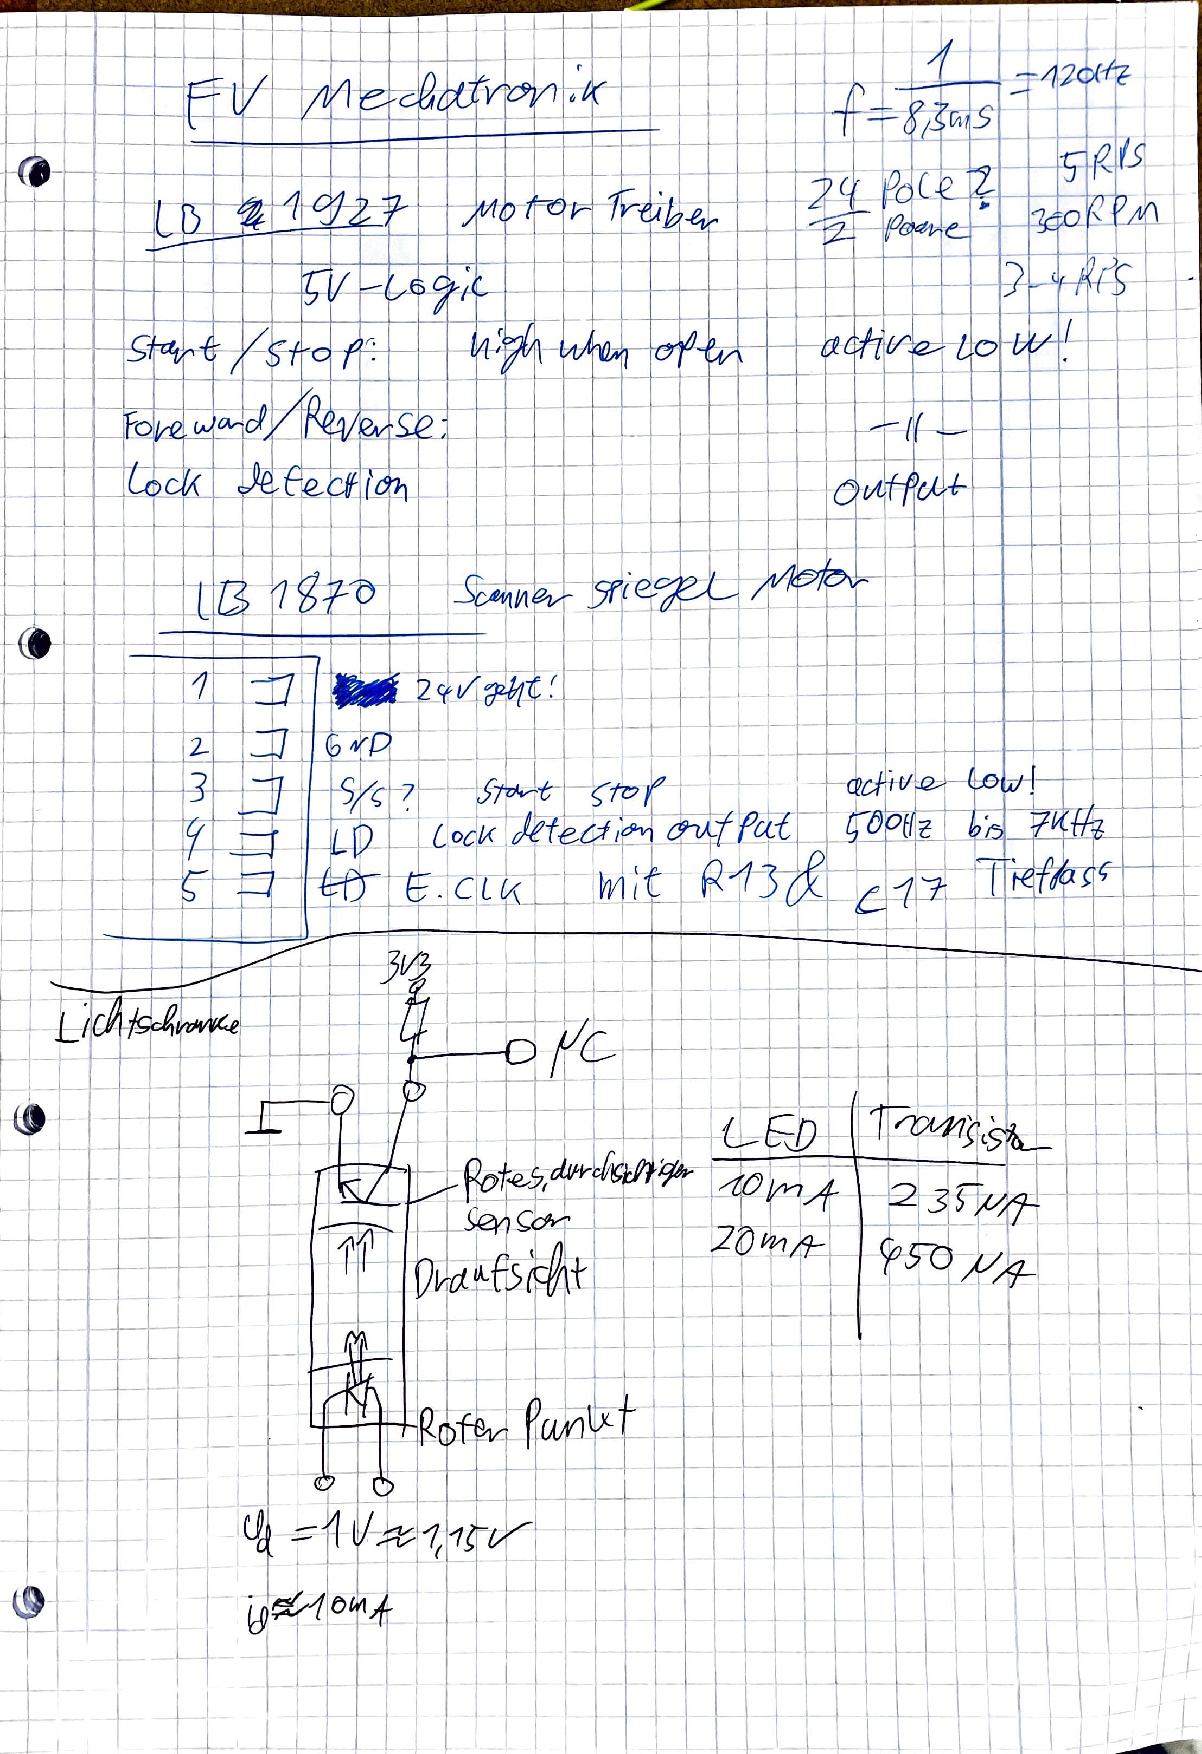
\includepdf[fitpaper=true]
{images/Lichtschranke}     %file name of title page


\chapter{Aufgabe}

Ziel der Übung ist es nun, eine Schreibmaschine mit den analysierten Komponenten zu bauen.
Ein Stift soll dabei entlang zwei Achsen bewegt werden, um auf einem Blatt Papier einen vom PC gesendeten Text in einer Schreibschrift zu schreiben.
Dabei ist auch ein Heben und Senken des Stiftes notwendig.

\chapter{Aufbau}

Die Führung des Stiftes erfolgt nach dem Core-XY-Prinzip über Linearführungen, die mit zwei Stepper-Motoren angetrieben werden.

Die Core-XY-Steuerung ist schematisch in Abbildung \ref{fig:corexy} dargestellt. Die Motoren bewegen die Achsen über zwei unabhängige Riemenschleifen.
Bewegen sich beide Motoren in die gleiche Richtung, bewegt sich der Stift entlang der waagrechten Achse.
Bewegen sich die Motoren in entgegengesetzte Richtungen, bewegt sich der Stift entlang der senkrechten Achse.
Bewegt sich nur ein Motor, bewegt sich der Stift diagonal.
Die diagonale Bewegung ist dabei stets eine Summe von Bewegungen entlang beider Achsen.
Wird ein Motor beispielsweise um 10 Schritte gedreht, während der andere feststeht, bewegt sich der Stift um 10 Schritte entlang beider Achsen,
also $10\cdot\sqrt{2}\approx 14.1$ Schritte diagonal.
Die Unabhängigkeit der Achsen entkoppelt deren Dynamik und ermöglicht eine präzise, verzerrungsarme Bewegung.

Das Heben und Seken des Stiftes erfolgt über einen Lorentz-Aktuator (VCA). Der Stift ist mit einer Feder nach oben vorgespannt, sodass er im unbestromten Zustand angehoben ist.
Wird der Aktuator mit Strom versorgt, wirkt eine Kraft nach unten, die den Stift auf das Papier drückt.

Der reale Aufbau ist in Abbildung \ref{fig:aufbau} zu sehen.

\bild{htb}{0.7}{images/corexy}{Core-XY-Steuerung}{fig:corexy}
\bild{htb}{0.7}{images/aufbau}{Aufbau der Schreibmaschine}{fig:aufbau}


\chapter{Spezifikationen}

Die minimale Auflösung der Maschene ist durch die Schrittweite der Stepper-Motoren gegeben. Im Fullstep-Betrieb beträgt die Schrittweite $\phi=7,5^{\circ}$.
Werden die Riemen direkt über eine Riemenscheibe mit $d=\qty{10}{\milli\meter}$ Durchmesser geführt, ergibt sich eine Schrittweite von ca. $d\pi\cdot\frac{\phi}{360^\circ}\approx \qty{0.65}{\milli\meter}$ entlang der beiden Achsen.
Die Auflösung entlang der Diagonalen beträgt damit ca. $\qty{0.93}{\milli\meter}$.

Im Halfstep-Betrieb ist die Schrittweite halb so groß und die Auflösung (entlang der Achsen) kann auf ca. \qty{0.33}{\milli\meter} erhöht werden.
Durch Microstepping mit PWM kann die Auflösung weiter erhöht werden, in der Praxis zeigt sich jedoch, dass dadurch eher die Linienqualität verbessert wird, während die tatsächliche Auflösung nicht wesentlich erhöht wird.

Für die realistische Auflösung des Systems ist die Mechanik ausschlaggebend. Aufgrund von Toleranzen und Spiel der Stifthalterung, Linearführungen und Riemen kommt es zu
Ungenauigkeiten, die die Auflösung auf ca. $\epsilon=\qty{1}{\milli\meter}$ begrenzen.


Die Geschwindigkeit der Maschine ist durch die maximale Schrittfrequenz der Stepper-Motoren begrenzt. Die Motoren können im Fullstep- und Halfstep-Betrieb mit bis zu ca. $f=\qty{200}{\hertz}$ betrieben werden.
Im Halfstep-Betrieb ergibt dies eine maximale Geschwindigkeit von ca. \qty{58}{\milli\meter\per\second} entlang der Achsen und \qty{41}{\milli\meter\per\second} entlang der Diagonalen.


Um die Spezifikationen zu überprüfen, wird ein Testmuster (sh. Abb.~\ref{fig:testmuster}) gezeichnet.
Es werden acht Linien in einem Sternmuster von außen zur Mitte gezeichnet, wobei die Linien jeweils um \qty{45}{\degree} zueinander versetzt sind.
Das Muster ist 200x200 Steps groß, was einer Länge der vier axialen Segmente von $\qty{29}{\milli\meter}$ und der vier diagonalen Segmente (100 + 100 Steps) von $\qty{41}{\milli\meter}$ entspricht.
Da der Stift von außen nach innen bewegt wird, beträgt die Gesamtstrecke $s=4\cdot 2 \cdot 100 + 4 \cdot 2 \dot 200 \,\text{Steps} = 2400 \,\text{Steps}$.

\textbf{Rahmenbedingungen:} Es wird eine weitgehend vibrationsfreie Umgebung angenommen. Es erfolgen keine Störungen durch z.B. Stöße. Das Papier ist
auf der Zeichenfläche mit Klebeband fixiert. Das Zeichnen erfolgt mit einem Fineliner. Dessen Strichstärke beträgt nominal \qty{0.4}{\mm}, aufgrund von Anpressdruck und
Verlaufen der Farbe ins Papier beträgt die Strichstärke real ca. \qty{1}{\mm} - gerade an der mechanischen Toleranz.
Da der Halfstep-Betrieb bereits hinreichend genau ist (Auflösung liegt deutlich unterhalb der mechanischen Toleranz), wird dieser Betriebsmodus für die Tests angenommen.

\begin{itemize}
\item \textbf{Genauigkeit:} Die Absolutgenauigkeit kann durch den Versatz der Linienenden in der Mitte des Sternmusters abgemessen werden. Dieser Versatz muss $\delta\le\qty{1}{\mm}$ betragen.
\item \textbf{Wiederholbarkeit:} Die Wiederholgenauigkeit wird durch mehrfaches Überschreiben des Musters gemessen.
Die Linien dürfen sich am Ende in keinem weiteren Radius als $\qty{1.25}{\mm}$ (mechanische Toleranz + Zusatztoleranz) von der ursprünglichen Linie bewegt haben.
\item \textbf{Geschwindigkeit:} Die Geschwindigkeit wird durch die Zeitmessung für das Zeichnen des Musters überprüft. Sie muss $t=\frac{s}{f}=\qty{12}{\second}\pm\qty{0.5}{\s}$ betragen.
\end{itemize}

Für einen Text in Schreibschrift mit einer Zeilenhöhe von ca. $\qty{10}{\milli\meter}$ wird eine Kurvenlänge von durchschnittlich $\qty{25}{\mm}$ pro Buchstabe angenommen.
Unter der Annahme, dass nur die Diagonalgeschwindigkeit erreicht werden kann, ergibt sich eine Schreibgeschwindigkeit von ca. $\frac{25}{41}\approx 0.6 \,\frac{\text{Buchstaben}}{\text{s}}$.

Der Text "Mechatronik und Instrumentierung" besteht aus 32 Zeichen (inklusive Leerzeichen) und wird damit in ca. \qty{19.5}{\s} geschrieben.

\bild{htb}{0.7}{images/test_pattern}{Testmuster}{fig:testmuster}

% \bibliographystyle{plain}
% \bibliography{Literatur}
\end{document}

